%!TEX root = ../thesis.tex
\chapter{Entropy Rate Estimation\label{ch:crossentropy}}

Extracting information flows is a problem deeply rooted in information theory. To examine these flows requires tools to quantify and measure this information in the form of natural language. As discussed in \autoref{ch:background}, the words used to construct language have no qualitative meaning in the context of the numerical analysis. This means that the tools are comparative in nature. Indeed, information theory has been used extensively to compare properties of information in language\cite{cite several papers, maybe add a bit more detail here}. 

In this chapter, we extend this philosophy in two key ways. We introduce a non-parametric entropy rate estimator and check it's assumptions using real data. We then generalise this entropy rate to a cross entropy rate, developing a tool for analysing information flows. 

\section{Entropy Rate Estimation}

Recall \autoref{def:entropyrate} of the entropy rate of a stochastic process. While a useful theoretical tool, this can be very difficult to compute, requiring knowledge of the joint entropy for a infinite set of realisations.

To overcome this, we seek a way to estimate the entropy of the process from a known sequence of data. In 1998 Kontoyianni et al. proved the convergence of a non-parametric entropy estimator in stationary processes~\cite{kontoyiannis_nonparametric_1998}.

\begin{definition}[Kontoyianni Entropy Rate] \label{def:kontoyianni}
	For a stochastic process $\mathcal{X} = \{X_i\}$, with $n$ realisations, the entropy rate is given by,
	\begin{equation}\label{eq:entropy:kontoyiannidef}
		H(\mathcal{X}) = \lim_{n\to \infty}\frac{n \log n }{\sum_{i=0}^n \Lambda_{i} },
	\end{equation}
	where  $\Lambda_{i}$ is the length of the shortest subsequence starting at position $i$ that does not appear as a contiguous subsequence in the previous $i$ symbols $X_{0}^{i}$. This can also be obtained by adding 1 to the longest match-length, 
	 \begin{equation}\label{eq:entropy:lambda}
	  \Lambda_{i}=1+\max \left\{l: X_{i}^{i+l}=X_{j}^{j+l}, 0 \leq j \leq N-i, 0 \leq l \leq N - i - j \right\}.
	 \end{equation}
\end{definition}

%<lit review>
This idea of using matched sub-sequences of text draws from the original work by Lempel and Ziv~\cite{ziv_universal_1977} in compression algorithms based on coding schemes. These algorithms attempt to compress a sequence down into the smallest possible representation, which at perfect efficiency would be the entropy, $H$. However these universal coding algorithms have no universal rate of convergence~\cite{shields_universal_1993, shields_universal_1995} and in practice other approaches are often employed, tailored to the specific application at hand.

The idea of an entropy estimator based on match lengths was originally put forward by Grassberger~\cite{grassberger_estimating_1989} and proved consistent for independent and identically distributed (i.i.d.) processes and mixing Markov chains~\cite{shields_entropy_1992}, stationary processes~\cite{kontoyiannis_prefixes_1994} and more generally to random fields~\cite{quas_entropy_1999}.


Wyner and Ziv~\cite{wyner_asymptotic_1989} showed that for every ergodic process the match length $\Lambda_{n}$ grows like $\frac{\log{n}}{H}$ in probability.  Extending from this notion Kontoyianni et al. showed the convergence of \autoref{eq:entropy:kontoyiannidef} in stationary ergodic processes using the match-length $ \Lambda_{i}$. This match-length in \autoref{eq:entropy:lambda} can be seen as the length of the next phrase to be encoded in the sliding-window Lempel–Ziv algorithm.

%<match lengths>
Conceptually, this match-length is simple. \autoref{fig:entropy:matchlength} shows the calculation of two match-lengths at different time points of a line from Doctor Seuss. At each index $i$, the elements immediately proceeding ($i, i+1, i+2, \dots$) are compared to the history of elements before $i$. The matches of length $k$ are found such that the elements from $j$ to $j+k$ perfectly match the elements from $i$ to $i+k$, for any $j<i$ where $k$ is then maximised. This search only considers the length of the match, regardless of it's location in the history. 

\begin{figure}[ht!]
	\centering
	\includestandalone[width=\textwidth]{chapter2/figs/tikz/lambda_count}
	\caption{An example calculation of the match-length based $\Lambda_i$ applied to a line from Green Eggs and Ham by Doctor Seuss. {\color{blue} Blue text} is that which has been matched from past to the future.\label{fig:entropy:matchlength}} 
\end{figure}
%</match lengths>

Even before it's formalisation by Kontoyianni et al., similar estimators had appeared in the literature applied to experimental data to determine the entropy rates of processes~\cite{chen_using_1993, chen_fast_1995, farach_entropy_1995, juola_what_1997}.
%</lit review>

% Final note
Moving forward we will assume any any discussion of the \emph{entropy rate} of a single process is assumed to be the \emph{Kontoyianni entropy rate} of that process, unless otherwise stated.


% ASSSUMPTIONS
\section{Assumptions of Entropy Rate Estimation}

The proof of convergence of this entropy rate places some limits on the process of investigation. In particular, three assumptions are made for convergence: ergodicity, stationarity and the Doeblin Condition (DC).

The Doeblin Condition is a reasonably weak condition, but is fundamental in the proof of the convergence. Simply put, the DC requires that after an arbitrary $r$ time steps, every state is possible again with positive probability~\cite{kontoyiannis_prefixes_1994}. More formally, the definition is as follows.

\begin{definition}[Doeblin Condition (DC)]
	There exists an integer $r\geq 1$ and a real number $\beta \in(0,1)$  such that,  for all  $x_{0} \in \mathcal{A}, \quad P\left\{X_{0}=x_{0} \mid X_{-\infty}^{-r}\right\} \leq \beta, $ with probability one. 
\end{definition}

Fortunately, as Kontoyianni et al. themselves state, the DC is ``certainly satisfied by natural languages''~\cite{kontoyiannis_nonparametric_1998}. Given the DC is not a fierce restriction, the condition is easy to satisfy. 

In contrast, the assumptions of ergodicity and stationarity are  harder to confirm. A long-standing assumption of information theory is that natural language can be modelled by a stationary process~\cite{shannon_mathematical_1948, shannon_prediction_1951, cover_elements_2012}. The assumption, while flawed, is well precedented and used again in this work.

While the much of the literature including the work of Kontoyianni assume ergodicity of natural language, some suggest that language should be modelled by a \emph{strongly nonergodic} stationary process~\cite{debowski_is_2018}. In brief, this contention is founded upon the idea that any given collection of text, such as a book, has a topic containing a small finite subset of words. Suggesting that it's text will inherently not explore the full state space of language. While well founded, our interest is not to look at the entropy rate of the English language as a whole, but rather to look at the entropy rate of individual text streams, which can explore the state space of news under consideration. As such, the assumptions of ergodicity and stationarity appear justified in the context of the problem.


%<Convergence>
\subsubsection{Convergence}
With the assumptions of the proof addressed, the challenges of entropy convergence needs to be examined. The entropy rate defined in \autoref{eq:entropy:kontoyiannidef} is based upon an infinite set of data to calculate $\Lambda_i$'s over. In reality, we have finite data, and need to examine the convergence of a modified estimator.

\begin{definition}[Kontoyianni Entropy Rate Estimator] \label{def:kontoyianni}
	The Kontoyianni Entropy Rate in \autoref{def:kontoyianni} can be estimated on a finite stochastic process $\mathcal{X} = \{X_i\}$, with $N$ realisations, by
	\begin{equation}\label{eq:estimate}
		\hat{h} = \frac{N \log N }{\sum_{i=0}^n \Lambda_{i} },
	\end{equation}
	where  $\Lambda_{i}$ is, as earlier, the length of the shortest subsequence starting at position $i$ that does not appear as a contiguous subsequence in the previous $i$ symbols $X_{0}^{i}$.
	 \begin{equation}
	  \Lambda_{i}=1+\max \left\{l: X_{i}^{i+l}=X_{j}^{j+l}, 0 \leq j \leq N-i, 0 \leq l \leq N - i - j \right\}.
	 \end{equation}
\end{definition}

To examine the convergence of the estimator, a model of language can be used to generate sequences of text, upon which we can estimate the entropy rate.

%<Zipf convergence>
\begin{figure}[h]
\centering
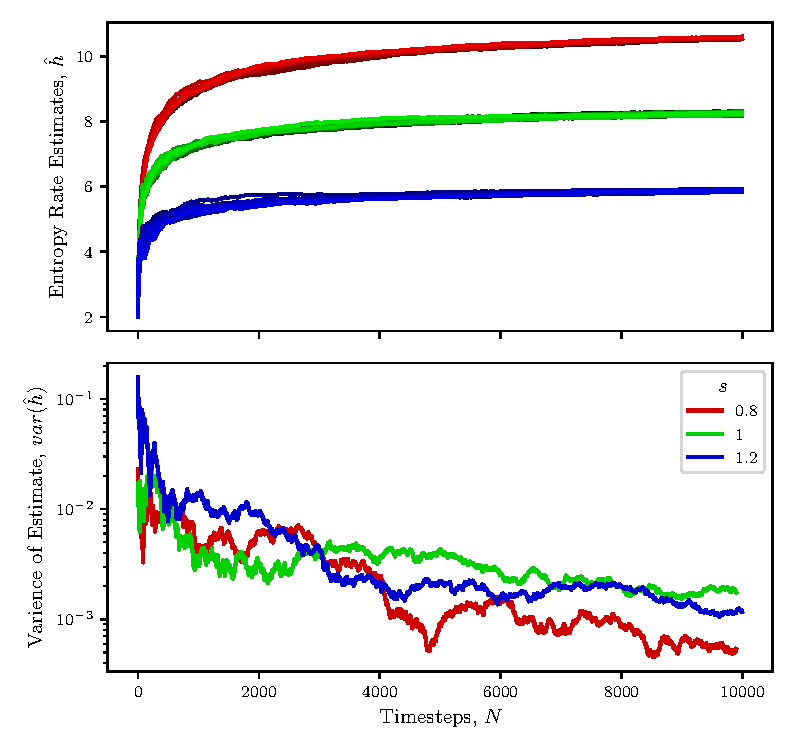
\includegraphics{chapter2/figs/Zipf_entropy_convergence.pdf}
\caption{Convergence of the Kontoyianni entropy rate estimator on sequences of i.i.d Zipf law realisations with varying Zipf law rates, $s$. \label{fig:entropy:zipfconvergence}}
\end{figure}


\autoref{fig:entropy:zipfconvergence} shows the convergence of the estimator for a set of i.i.d realisations of a Zipf's law distribution. As discussed in \autoref{sec:textgeneration}, Zipf's law is a common tool for generating simple text due to it's similarity to the power-law distributions of vocabulary seen in real corpora. The Zipf's law can be used with a number of exponents, $s$, where larger exponents tighten the distribution, reducing the observed vocabulary size of the sequence and hence the entropy. 

Sequences are generated with 30,000 i.i.d realisations of the Zipf's law and the entropy rate of estimate of the process is calculated at each timestep between 1 and 30,000 using \autoref{eq:estimate} applied to only the realisations before that timestep. Estimates of entropy start very low when few realisations are available and rapidly rise as new realisations add complexity. Within the first few hundred timesteps entropy estimates can vary between timesteps as new realisations are added matching or not-matching previous realisations. This is reflected in the high variance between entropies estimates for Zipf process with the same exponent in these early stages. As the number of timesteps included reaches 5000 to 7500 the bias and variance of the estimate are significantly reduced and begin plateauing. 

As more timesteps are added, the estimator continues to converge to the asymptotic entropy and the variance between estimates continues to reduce. High complexity sequences take longer to converge to this entropy, but achieve suitably small levels of bias and variance within 15000 timesteps even for high entropy sequences. This is an important finding given the speed of calculating these estimates. The algorithm to calculated the match-lengths needed for estimating the entropy is $O(n^3)$ time complexity. As a result, speed takes a significant hit as the number of timesteps is increases. When performing simulations a parsimonious choice of simulation length is advantageous in allowing multiple simulations to be run. Hence, for Zipf law distributions a simulation length of 15000 is deemed sufficient for convergence to the entropy.
%</Zipf convergence>


%<Zipf real entropy>
To confirm the validity of this approach, we can examine the known entropy rate of the Zipf processes. As shown in \autoref{proof:iidentroptrate}, the entropy rate of an i.i.d process is simply the entropy of each element. In the case of a Zipf law the distribution has entropy\footnote{
	Proof: The probability of a word of rank $k$ being selected from a pool of $N$ elements using exponent $s$ is $(k^s H_{N,s})^{-1}$. Hence, the entropy of each individual element is $\sum_{k=1}^N  (k^s N_{N,s})^{-1} \ln\left( (k^s N_{N,s})^{-1} \right)$. Using $H_{N,s} = \sum_{k=1}^N \frac{1}{k^s}$, this can be rearranged to $\frac{s}{H_{N, s}} \sum_{k=1}^{N} \frac{\ln (k)}{k^{s}}+\ln \left(H_{N, s}\right)$. }, 
\begin{equation}
	\frac{s}{H_{N, s}} \sum_{k=1}^{N} \frac{\ln (k)}{k^{s}}+\ln \left(H_{N, s}\right)
\end{equation}
where $H_{N,s}$ is the Nth generalized harmonic number defined by, $H_{N,s} = \sum_{k=1}^N \frac{1}{k^s}$. Many approaches to calculating this entropy use the asymptotic entropy as $N \to \infty$. This draws on the result that $\lim_{N\to \infty} H_{n,s} = \zeta(s)$, where $\zeta$ is the Riemann zeta function. While this asymptotic approach works well for numbers well above 1, the Riemann zeta function explodes to infinity at $s \to 1$. As such, the analytic entropy degenerates as $s \to 1$ and is poorly defined for $s < 1$. In contrast, using a finite choice of $N$ results in well defined processes and entropies for all $s >0$. A choice of $N=199338$ is made to match the observed total vocabulary size seen in the news-media Twitter data as explored in \autoref{sec:vocabsizes}. For high values of $s$, the two asymptotic and finite entropies are very close, 3.18158 and 3.18368 respectively, and only differ significantly as $s$ approaches 1. This finite entropy calculation allows the model to more accurately match the Zipf exponents fitted to real text data, which are often closer to or below 1~\cite{williams_text_2015}.


% <Simulations>
Using simulations of the Zipf process for a variety of values of the exponent $s$, we compare how the estimated entropy rate compares to the `true' entropy rate as calculated above. In \autoref{figs:entropy:convergencetotruth} simulations are run for values of $s$ in the range [0.01, 2] with increments of 0.01. 
High values of $s$ in this range have an increasingly lower entropy, as the skewness of the distribution becomes more extreme. This distribution results in a high numbers of realisations of low rank words creating repeated sequences which lower both the analytic entropy rate and the entropy rate estimate. Values above 2 reduce the entropy rate in vanishingly smaller increments. 

\begin{figure}[ht!]
\centering
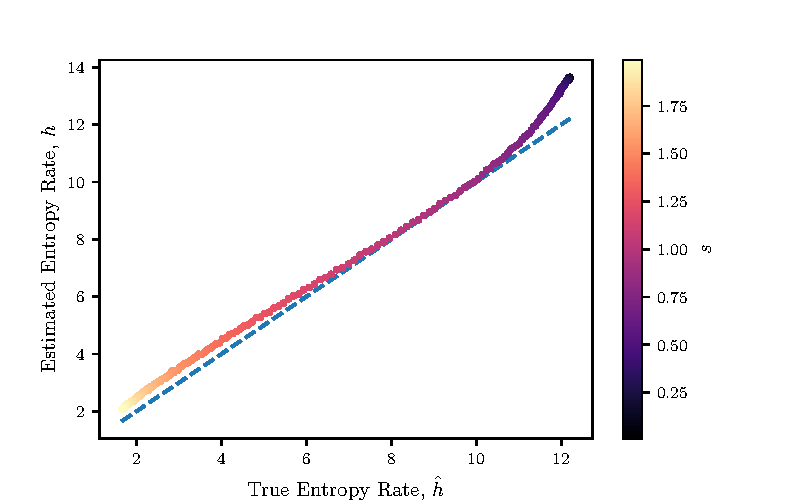
\includegraphics{chapter2/figs/convergence_to_truth.pdf}
\caption{Estimated entropy rates and analytic entropy rates of sequences of 20,000 i.i.d Zipf law random variables with exponent $s$. Dashed line represents the true entropy rate equalling the entropy rate estimate. As values for $s$ approach 0 the high variance of the distributions results in poor estimates due to the finite sample of the Zipf law. \label{figs:entropy:convergencetotruth}}
\end{figure}

For values of $s$ between 2 and 0.5, the entropy rate estimate appears to be a rough upper bound on the true entropy rate of the process. This upper bound is only achieved with sufficient lengths of sequences such that the estimator can converge to this upper bound. Indeed, given sufficient length the variance of the estimates on sequences drawn from the same distribution is very low. This is in contract to the bias of the estimate, which varies with the changing exponent. 

When $s$ becomes lower than 0.5, the Zipf law distribution becomes more evenly distributed with reduced skew. This results in a larger probability of low rank word occurrences, producing a process where many words appear very few times. As a result, the finite nature of the sequence results in a entropy rate estimate that grows faster than the true entropy, increasing the bias for these high entropy sequences. 

In general, the convergence of the estimator is sufficient, with a slight caveat. While the estimator convergences to an estimate tightly with very little variance, the bias of the estimate is not constant and varies with the complexity of the sequences. While this finding is itself interesting and warrants future work, the estimator is both consistent and it's estimates appear monotonic with the true entropy rate. As such, we will use this estimator to approximate the true entropy rate moving forward, with a cautious eye to the possible effects of this inconsistent bias. 
%</Zipf real entropy>

%<Real data entropy convergence>
To extend from this result using the Zipf law process, we apply the same approach using the news-source Twitter data. 5000 tweets are drawn uniformly from the collection of all tweets from all news-media outlets. These tweets are tokenized and concatenated into a single sequence of natural language text ranging from 85000 tokens to 90000.

Unlike the case of Zipf, we cannot show a true entropy rate for this distribution, but can demonstrate it's convergence.  Each sample has the entropy rate calculated using only the first $N$ tokens, up to the length of 60,000 tokens. \autoref{fig:entropy:realconvergence} shows the clear convergence of the estimator of the real data, approaching a entropy rate of 7.53. As with the Zipf simulations, the variance of the estimated entropy rates of the samples reduces as more tokens are included in the estimate.  The real data takes longer to converge, needing up to 50,000 tokens to achieve a variance of less that $10^{-3}$.

\begin{figure}
\centering
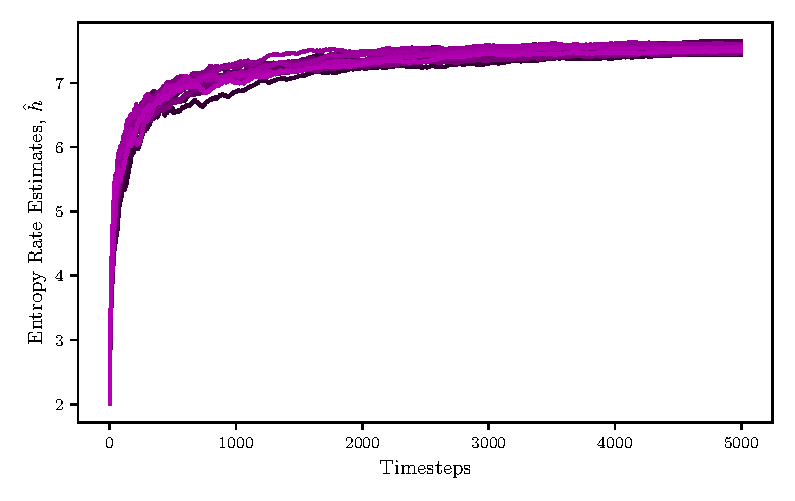
\includegraphics{chapter2/figs/real_entropy_convergence.pdf}
\caption{Convergence of the Kontoyianni entropy rate estimator on sequences words generated by drawing tweets uniformly without replacement from the pool of all tweets produced by all news-media organisations. \label{fig:entropy:realconvergence}}
\end{figure}

%</Real data entropy convergence>

%<Tikz of flow>
\subsubsection{Self Entropy Rate Summary}

\begin{figure}[ht!]
	\centering
	\includestandalone[width=\textwidth]{chapter2/figs/tikz/self_flow}
	\caption{A conceptual diagram of self entropy rate estimation using the Kontoyianni entropy rate estimation. Tweets shown as blue rectangles are positioned in time and contain textual content. Content proceeding the position \emph{Now} will have snippets of text matched with text from the history of the process, denoted by {\color{orange}orange} and \underline{unlined} text. These text matches are used to calculate the $\Lambda_i$'s which inform the entropy estimate. \label{fig:entropy:selfflow}} 
\end{figure}

Before moving away from the self entropy rate, let's take one more opportunity to visualise the how this Kontoyianni entropy rate estimator works in the real data. \autoref{fig:entropy:selfflow} shows a simplified version of the conceptual self entropy rate calculation. For a given Twitter user, tweets appear sequentially, separated in time. At any given time, the content of the immediate future of that user's tweets is compared to the entire history of the tweets before that time. This process is then repeated for all possible times in the data. In essence, the calculation of the $\Lambda_i$'s is a repeated examination of how much of the immediate complexity at timestep $i$ can be described using the history of the sequence. In total, this estimator provides an average of how many bits are needed to describe the future of this process given it's past at any point.

%% Histogram of self entropy rates ??

%</Tikz of flow>

\section{Cross Entropy Rate}

To create a notion of information flow, we need to move beyond looking at individual sources in isolation. To do so, we need a tool of comparison between sources rooted in our tools from information theory. We find such a tool in a generalisation to a Kontoyianni cross entropy rate.

Similar to the extension of entropy, $$H(X) = \sum_{x \in \mathcal{X}} p(x)\log p(x)=-\mathbb{E}[\log P(X)]$$ to cross entropy, $$H(p,q) = \sum_{x \in \mathcal{X}} p(x)\log q(x) = -\mathbb{E}_p[\log q(X)],$$  in \autoref{def:crossentropy}, we can generalise our notion of Kontoyianni entropy rate from \autoref{def:kontoyianni} to a \emph{cross} entropy rate which we will call the Kontoyianni cross entropy rate.

\begin{definition}[Kontoyianni Full Cross Entropy Rate]
	The cross entropy rate of a {\color{target} target process} $\mathcal{T}$ coded from a {\color{source} source process} $\mathcal{S}$ can be estimated via,
	\begin{equation}
	H(\mathcal{T} || \mathcal{S})=\frac{N_{\mathcal{T}} \log _{2} N_{\mathcal{S}}}{\sum_{i=1}^{N_{\mathcal{T}}} \Lambda_{i}(\mathcal{T}| \mathcal{S})}
	\end{equation}
	Where $N_{\mathcal{X}}$ is the length of process $\mathcal{X}$ and $\Lambda_{i}(\mathcal{T}| \mathcal{S})$ is given by the shortest subsequence starting at position $i$ in the {\color{target}target} $\mathcal{T}$ that does not appear as a contiguous subsequence anywhere in the {\color{source}source} $\mathcal{S}$.
	\begin{equation}
	\Lambda_{i}(\mathcal{T}| \mathcal{S}) = \max \left\{l: T_i^{i+l}=S_{j}^{j+l}, 0 \leq j \leq N_{\mathcal{S}},  0 \leq l \leq \min( N_{\mathcal{S}}- j , N_{\mathcal{T}}- i )\right\},
	\end{equation}
	where $T_a^{b}$ and $S_a^b$ are continuous subsequences starting from index $a$ to index $b$ of the {\color{target} target}, $\mathcal{T}$, and  {\color{source} source}, $\mathcal{S}$, processes respectively.
\end{definition}

This approach to a cross entropy matches segments of text in the {\color{target}target} to segments of text anywhere in the {\color{source}source} in the same manner that the Kontoyianni entropy rate matched segments of text in the future of a process from a index, $i$, to the history before the index. In contrast to the entropy rate estimate, which asking how much information was needed on average to \emph{describe the future of a source from it's past}, this cross entropy rate estimate is asking how much information is needed on average to \emph{describe the target given full knowledge of the source}. 

\begin{figure}[h!]
	\centering
	\includestandalone[width=\textwidth]{chapter2/figs/tikz/unsynced_flow}
	\caption{A conceptual diagram of \textbf{Kontoyianni full cross entropy rate} estimation. Tweets shown as rectangles are positioned in time for both a target and source, containing textual information. Content in the {\color{source}source} is matched with content in the immediate future of the {\color{target}target} for a given time point, $t$, to calculate match-lengths. This time point is shifted along the {\color{target}target} timeline to average match-lengths and calculate the full cross entropy rate.\label{fig:entropy:unsyncedflow}} 
\end{figure}

This full knowledge over all of the process gives the estimator the `Full' in it's title, but presents a impropriety. In the context of our problem, this estimator is cheating by viewing the future of news through the lens of the source process. 

As \autoref{fig:entropy:unsyncedflow} illustrates, the text subsequence match in the target could be drawn from future time points in the source. Restated, the cross entropy rate will, in-part, be describing how much information you need to encode the future of a piece of target news already knowing the future of the news from another source. While this may be an interesting insight in itself, it doesn't probe the underlying process of \emph{information flow} with which this thesis focuses. 

Rather than looking at the entire lifetime of the source during the matching calculations, we can reduce our search space to the text that occurred in the \emph{past} of the source. To achieve this we use an important piece of our data, the time that tweets occurred. For each word in the target process, $T_i$ has an associated time with it, $t(T_i)$. When matching the future of $\mathcal{T}$, starting from an index $i$, we can reduce the source process, $\mathcal{S}$ to only the words that were themselves tweeted before time $t(T_i)$. 

Put simply, we can alter the Kontoyianni full cross entropy rate to a time-synced cross entropy rate by replacing the full {\color{source}} process, $\mathcal{S}$, with a time reduce source process $\mathcal{S}_{ \leq t(T_i)}$. This can be seen visually in \autoref{fig:entropy:timesyncedflow} and is formally defined as follows.

\begin{definition}[Kontoyianni Time-synced Cross Entropy Rate]
	The time-synced cross entropy rate of a {\color{target} target process} $\mathcal{T}$ coded from a {\color{source} source process} $\mathcal{S}$ can be estimated via,
	\begin{equation}
	H(\mathcal{T} || \mathcal{S})=\frac{N_{\mathcal{T}} \log _{2} N_{\mathcal{S}}}{\sum_{i=1}^{N_{\mathcal{T}}} \Lambda_{i}(\mathcal{T}| \mathcal{S}_{\leq t(T_i) } )}
	\end{equation}
	Where $\Lambda_{i}(\mathcal{T}| \mathcal{S}_{\leq t(T_i) })$ is given by the shortest subsequence starting at position $i$ in {\color{target}target} $\mathcal{T}$ that does not appear as a contiguous subsequence in the time reduced {\color{source}source} $\mathcal{S}_{\leq t(T_i) }$ where,
	\begin{equation}
	\mathcal{S}_{\leq t(T_i) } = \{S_j | t(S_j) \leq t(T_i) \forall i \}.
	\end{equation}
	Which gives,
	\begin{align*}
	\Lambda_{i}(\mathcal{T}| \mathcal{S}_{\leq t(T_i)}) = \max \{l: T_i^{i+l}=S_{j}^{j+l}, 0 \leq j \leq N_{\mathcal{S}},  \\  0 \leq l \leq \min( N_{\mathcal{S}}- j , N_{\mathcal{T}}- i ) \},
	\end{align*}
	where $T_a^{b}$ and $S_a^b$ are continuous subsequences starting from index $a$ to index $b$ of the {\color{target} target}, $\mathcal{T}$ process, and the time reduced {\color{source} source}, $\mathcal{S}_{\leq t(T_i)}$, respectively.
\end{definition}

\begin{figure}
	\centering
	\includestandalone[width=\textwidth]{chapter2/figs/tikz/timesynced_flow}
	\caption{A conceptual diagram of \textbf{Kontoyianni time-synced cross entropy rate} estimation. Tweets shown as rectangles are positioned in time for both a target and source, containing textual information. Content in the {\color{source}source} that occurs before time $t$ is matched with content in the immediate future of the {\color{target}target} from $t$ to calculate match-lengths. This time point is shifted along the {\color{target}target} timeline to average match-lengths and calculate the time-synced cross entropy rate.\label{fig:entropy:timesyncedflow}} 
\end{figure}


% Informantion flow idea
This time-synced entropy rate is testing not just the differences in the language processes of the source and target, but also measuring what information in the target is present in the source's history. This is an important distinction, as it allows us to probe a very important aspect of our data, namely, the time in which news is created. 

If a piece of information appears earlier in the source than in the target, it will be detected during the match length search, resulting in a lower entropy. This is to say, in the context of news, if the {\color{source}source} breaks a story first, \emph{less} information is required to describe the subsequent news output from the {\color{target}target}. 

Conversely, if a {\color{target}target} produces a piece of information before the {\color{source}source}, then that information will not appear in the history of the time-synced source during the match-length search. This will result in lower values of $\Lambda_i$ for that piece of information, which raises the cross entropy rate.

From this, we can find that, on average, if a {\color{source}source} produces information earlier than a {\color{target}target}, the cross entropy rate, $\hat{h}(\mathcal{T} | \mathcal{S})$, will be lower than if the {\color{target}target} produces information earlier than the {\color{source}source}. This method of examining who produces information first can be extended into a notion of \emph{information flow}, a discussion we will leave for \autoref{ch:quotermodel}.


\subsection{Validating the Assumptions Cross Entropy Estimation}

To validate these new cross entropy rate estimators a similar process is performed as with the entropy rate. Fortunately, many of the assumptions transfer over neatly.

In the case of ergodicity, stationarity and the Doeblin Condition, all three are properties of the process under investigation, which we argued above are well founded. We introduce a additional condition on the processes for the sake of cross entropy rates, namely that the processes have the same state space. This additional condition extends the earlier conditions to apply jointly between both the source and target processes. While not all news-media Twitters will have the same realisations of word in the corpus, the processes could be reasonably thought to have the same state space, as all process are using English and discussing similar topics.

This then leads naturally to the next question of convergence. Following a sample process of uniform withdrawals from a distribution will result in functionally similar convergence to the entropy rate above. Indeed, this can be seen in \autoref{fig:entropy:realcrossconvergence}, where tweets are sequences are draw uniformly from the pool of all tweets and cross entropy rates, denoted $\hat{h}_{\times}$ to distinguish from the entropy rate estimates $\hat{h}$, are calculated. This figure is, as expected, functionally similar to \autoref{fig:entropy:realconvergence} from the entropy rate section above. The cross entropy rate calculation is fundamentally no different from the entropy rate calculation as a randomly selection history of another process is just a useful and a randomly selected history of another process when both draw from the same distribution.


\begin{figure}
	\centering
	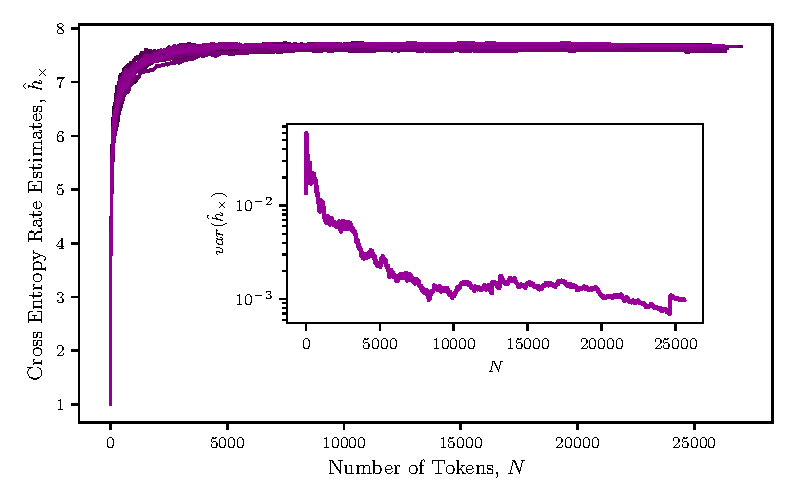
\includegraphics{chapter2/figs/cross_real_entropy_convergence}
	\caption{Convergence of the Kontoyianni time-synced cross entropy rate estimator on pairs of sequences independently generated by drawing tweets uniformly without replacement from the pool of all tweets produced by all news-media organisations.} \label{fig:entropy:realcrossconvergence}
\end{figure}

A more nuanced investigation of the cross entropy convergence emerges when we utilise processes with \emph{different} distributions. \autoref{fig:entropy:zipfcrossconvergence} does exactly this. Using pairs of exponents for different Zipf distributions simulations of 30,000 long i.i.d processes are made with separate target and source processes. The cross entropies rates are estimated across these pairs. When the exponents are equal, $s_{source}=s_{target}$, we observe the same entropy and convergence pattern as we would for a single i.i.d process with that exponent. 

When $s_{source} \neq s_{target}$ the entropy rates vary, and are not always similar to the entropy rate of the target or the source. 
% talk more

\begin{figure}
	\centering
	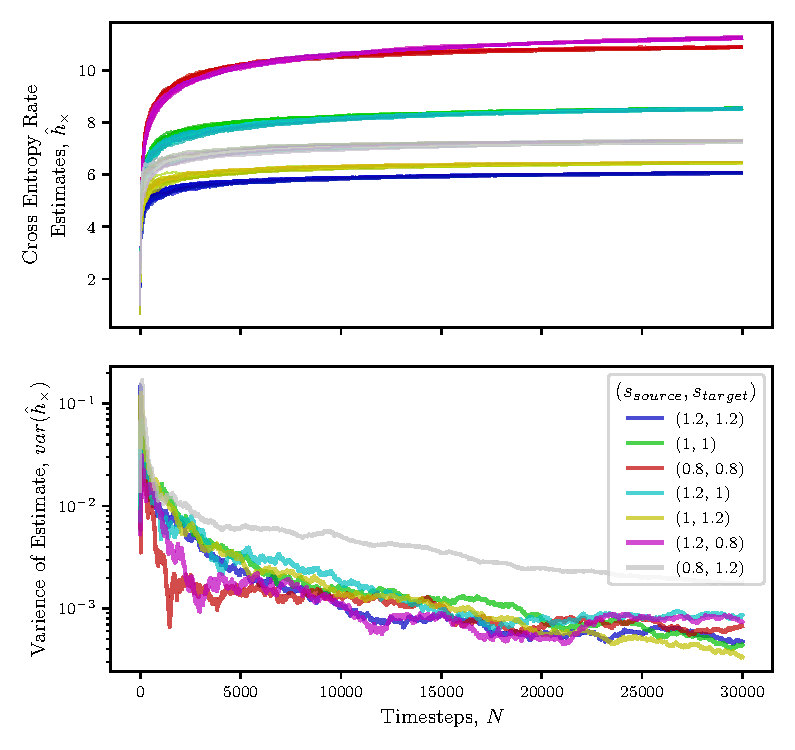
\includegraphics{chapter2/figs/cross_Zipf_entropy_convergence}
	\caption{Convergence of the Kontoyianni time-synced cross entropy rate estimator on pairs sequences of i.i.d Zipf law realisations with varying pairs of Zipf law rates, $s_{source}$ and $s_{target}$. } \label{fig:entropy:zipfcrossconvergence}
\end{figure}



\subsection{Predictability}
Perhaps this would be a good place to generalise the notion of cross maximal predictability.


\subsection{A Note on Package Development}

As stated earlier, a key challenge in estimating these Kontoyianni cross entropy rates is calculation speed. With time complexities of $O(n^3)$ on the number of input tokens, fast code is necessary to allow for estimation using long sequences. To achieve this speed and contribute to this field of work more broadly, a speed-focused open source package was developed to help researchers efficiently and easily calculate entropy rates such as those discussed above. The important snippets from code contributions of the package are available in \autoref{app:code} and this section will outline two key tools used in speeding the code up.

The fundamental complexity limitations of the algorithm mean that speed improvements need to come from smart implementation. Two techniques used are interesting enough to discuss briefly here, hashing and JIT compiling.

In the context of analysing language like a process, each word is simply an element of the state space. As such each word can be assigned a unique number to represent it's position in the state space. In doing so it allows the computations of the $\Lambda_i$'s to be performed using my faster integer operations. In practice developing such a lookup table for each word in the state space is slow and unnecessary. In the ProcessEntropy package, words are converted to 32 bit unsigned integers using Fowler–Noll–Vo hashing. Fowler–Noll–Vo is a non-cryptographic hash function which is very fast to compute. This converts each words to the same integer every time, with almost no collisions. 

I'm thinking of putting a section here that just talks about the need for speed of computation and highlights some of the tricks used to speed it up. E.g. Fowler–Noll–Vo hashing, JIT compiling. Do you think this is appropriate to include and if so at what level of detail. 

% \subsubsection{Hashing Tokens}

% speed comaprisons


\begin{figure}[h]
\centering
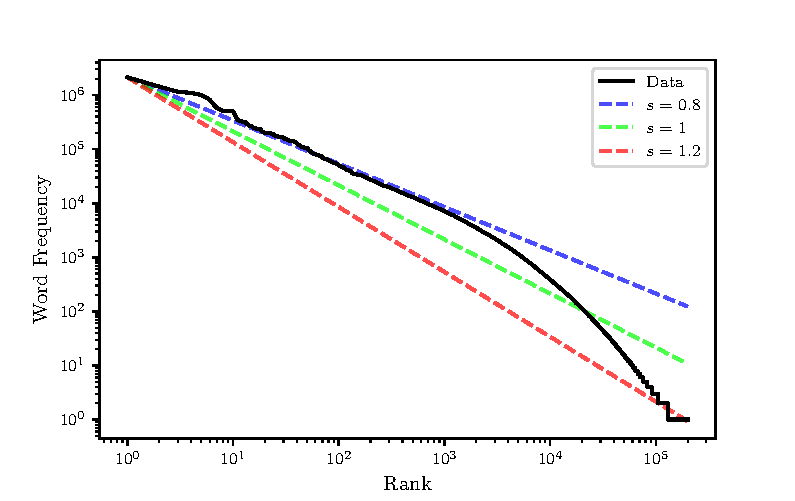
\includegraphics{chapter1/figs/fitted_zipf.pdf}
\caption{\ts{Bonus: Included for your reviewing, this is a figure that will soon be added to the data chapter.}  Word frequency of tokens in the corpus of all tweets produced by all news sources compared the rank of the token by frequency. Zipf law distributions are also shown for varying exponents, $s$. \label{fig:data:fitted_zipf}}
\end{figure} 

